% Non-rotated pendulum

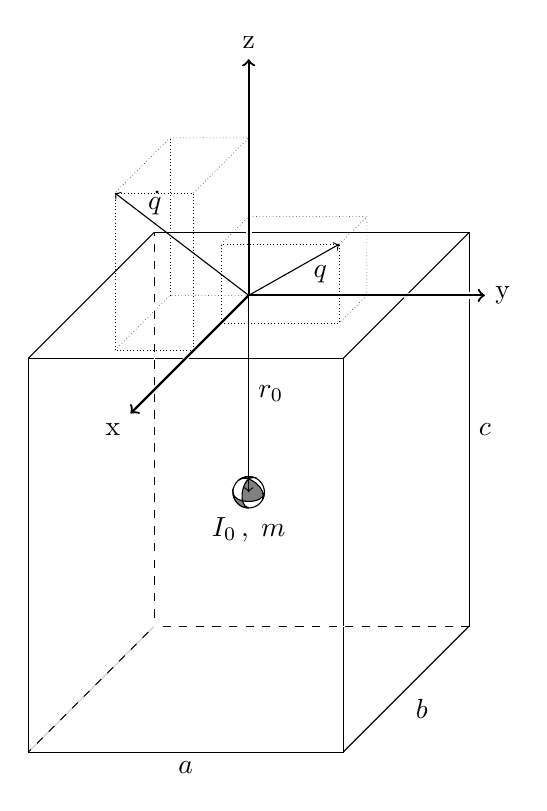
\begin{tikzpicture}
    % prism
    \draw (-2.8, -0.8) -- ( 1.2, -0.8) -- ( 1.2, -5.8) -- (-2.8, -5.8) -- cycle;
    \draw (-1.2,  0.8) -- ( 2.8,  0.8) -- ( 2.8, -4.2) -- (-1.2, -4.2) -- cycle;
    \draw (-2.8, -0.8) -- (-1.2,  0.8);
    \draw ( 1.2, -0.8) -- ( 2.8,  0.8);
    \draw ( 1.2, -5.8) -- ( 2.8, -4.2);
    \draw (-2.8, -5.8) -- (-1.2, -4.2);
    % back walls
    \draw[white, dashed] (-1.2, -4.2) -- (-2.8, -5.8);
    \draw[white, dashed] (-1.2, -4.2) --( 2.8, -4.2);
    \draw[white, dashed] (-1.2, -4.2) -- (-1.2,  0.8);
    % interupts at axis lines
    \draw[white] (-0.84, -0.8 ) -- (-0.76, -0.8 );
    \draw[white] (-0.04,  0.8 ) -- ( 0.04,  0.8 );
    \draw[white] ( 1.97, -0.03) -- ( 2.03,  0.03);
    \draw[white] ( 2.8 , -0.04) -- ( 2.8 ,  0.04);

    % lengths of sides
    \draw (-0.8, -5.8) node[anchor = north] {$a$};
    \draw ( 2.0, -5.0) node[anchor = north west] {$b$};
    \draw ( 2.8, -1.7) node[anchor = west] {$c$};

    % centre of mass
    \draw ( 0.0, -2.5) circle[radius = 0.2];
    \filldraw[fill=gray] ( 0.0, -2.7) arc[radius=0.2, start angle=270, end angle=180] to[bend right=90] ( 0.2, -2.5) to[bend left=10] ( 0.173, -2.6) to[bend right=80] (-0.13, -2.347) to[bend left=25] ( 0.07, -2.313) to[bend right=90] ( 0.0, -2.7);
    \draw ( 0.0, -2.7) node[anchor = north] {$I_{0} \,,\; m$};

    \draw[->] ( 0.0, 0.0) -- ( 0.0, -2.5);
    \draw ( 0.0, -1.25) node[anchor = west] {$r_{0}$};

    % coordinates
    \draw[thick, ->] (0, 0) -- (-1.5, -1.5) node[anchor = north east] {x};
    \draw[thick, ->] (0, 0) -- (3, 0) node[anchor = west] {y};
    \draw[thick, ->] (0, 0) -- (0, 3) node[anchor = south] {z};

    % q
    \draw[->] ( 0.0, 0.0) -- ( 1.15, 0.65);
    \draw ( 0.7, 0.5) node[anchor = north west] {$q$};
    \draw[densely dotted, very thin] (-0.35, -0.35) -- ( 1.15, -0.35) -- ( 1.15,  0.65) -- (-0.35,  0.65) -- cycle;
    \draw[densely dotted, very thin] (-0.35,  0.65) -- ( 0.00,  1.00) -- ( 1.50,  1.00) -- ( 1.50,  0.00) -- (1.15, -0.35);
    \draw[densely dotted, very thin] ( 1.15, 0.65) -- ( 1.5 , 1);

    % dot{q}
    \draw[->] ( 0.0, 0.0) -- (-1.7, 1.3);
    \draw (-1.4, 0.9) node[anchor = south west] {$\dot{q}$};
    \draw[densely dotted, very thin] (-0.70, -0.70) -- (-1.70, -0.70) -- (-1.70,  1.30) -- (-0.70,  1.30) -- cycle;
    \draw[densely dotted, very thin] (-0.70,  1.30) -- ( 0.00 , 2.00) -- (-1.00 , 2.00) -- (-1.70, 1.30);
    \draw[densely dotted, very thin] (-1.70, -0.70) -- (-1.00,  0.00) -- ( 0.00,  0.00);
    \draw[densely dotted, very thin] (-1.00,  0.00) -- (-1.00,  2.00);
\end{tikzpicture}
